\documentclass[a4paper,11pt]{article}
\usepackage[portuguese]{babel}
\usepackage{geometry}
\usepackage{graphicx}
\pagenumbering{arabic}
\usepackage{multicol}
\usepackage{hyperref}
\usepackage{float}

\geometry{a4paper, left= 1 cm, right= 1 cm, top= 1.5 cm, bottom= 1.5 cm}
\title{\textbf{Finanças pessoais}}
\author{Isaura Sofia Xavier Cid \\ 63761 - fc63761@alunos.fc.ul.pt \\ TP18 - Licenciatura em Engenharia Informática}
\date{}

\begin{document}

\maketitle
\begin{figure}[h]
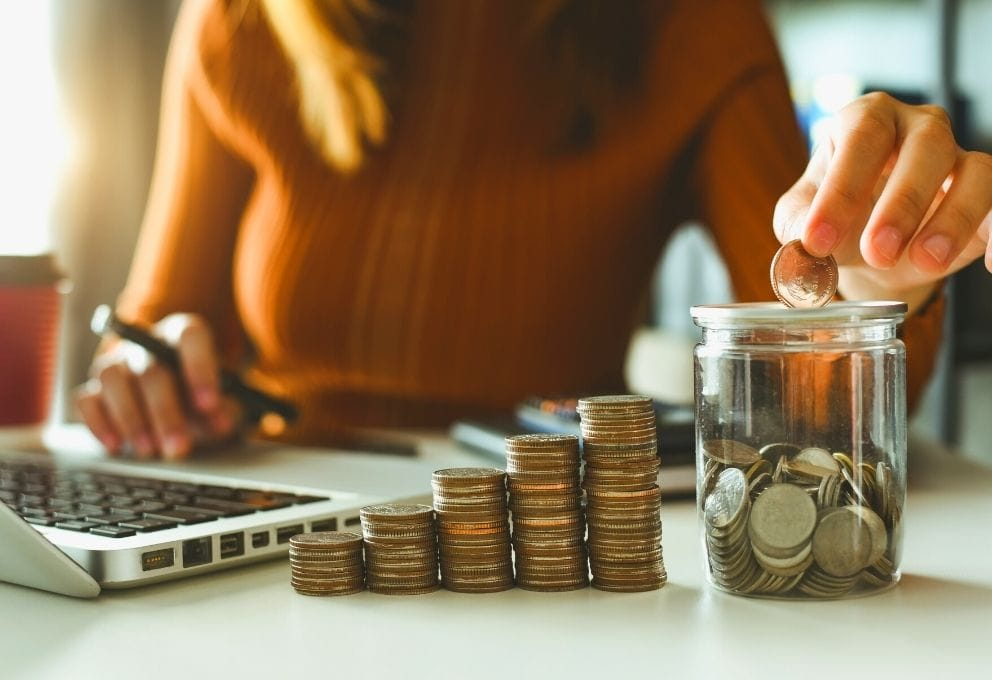
\includegraphics[scale=0.55]{finanças_pessoais.jpg}
\end{figure}
\thispagestyle{empty}

\newpage
\section{Índice}
\setcounter{page}{1}
\pagenumbering{roman}
\tableofcontents
\listoftables
\listoffigures

\pagenumbering{arabic}
\setcounter{page}{2}
\newpage
\section{Introdução}
\begin{multicols}{2}
As finanças pessoais são a prática de modos que contribuem para a gestão dos gastos de uma pessoa. A forma como gerimos o dinheiro impacta diversas áreas da nossa vida. Esta gestão permite o aumento do nosso bem-estar. Desta forma, é necessário haver \textbf{parâmetros} para a organização/gestão. Esses parâmetros podem ser, por exemplo: gastos essenciais, desejos pessoais, investimentos, dívidas, etc. Claro que, dentro destes, podem haver \textbf{sub-parâmetros}. Por exemplo, os \underline{gastos essenciais} incluem: casa, alimentação, saúde, gasolina, educação, etc. \\ \\É importante ainda, se possível, poupar uma parte do dinheiro mensalmente (para eventuais emergências, ou mesmo para satisfação pessoal).\\ \\ \textbf{É necessário e benéfico, então, uma educação financeira pessoal!} \\ \\
\underline{Sucintamente}, é importante:
\begin{itemize}
\item analisar e apontar os gastos mensais;
\item definir os principais objetivos financeiros;
\item cortar nos gastos desnecessários;
\item gastar com consciência, fazendo as seguintes perguntas:
\begin{enumerate}
\item É mesmo necessário?
\item Qual a utilidade que vou dar, a longo prazo?
\item Vai impedir de pagar algo mais necessário?
\item Tenho outras prioridades ou esta é uma prioridade suprema?
\end{enumerate}
\item ir acompanhando sempre o estado financeiro para:
\begin{enumerate}
\item a eventualidade de emergências;
\item investir.
\end{enumerate}
\item poupar mensalmente uma parte do salário;
\item educar-se financeiramente;
\item manter o orçamento pessoal atualizado.
\end{itemize}
\textbf{Sobre o último ponto}, manter o orçamento atualizado tem extrema importância. Isto significa que, de x em x tempo (definido pela pessoa), as finanças pessoais são revistas, ou seja, todos aqueles parâmetros são revistos e/ou atualizados (cortar, adicionar ou manter).
\end{multicols}
Tal como disse Thomas J. Stanley, "Plan your expenditures and your earnings will come more easily", que, traduzido, significa "Planeia os teus gastos e os teus ganhos chegarão mais facilmente". Um bom planeamento financeiro facilita o processo de ganho e gestão do dinheiro.

\newpage
\section{Caso de Estudo}
Neste caso, irei estudar o papel e a influência que um orçamento pessoal tem, demonstrando assim também como planear e organizá-lo. Através de tabelas e gráficos, observar-se-á que construir um orçamento pessoal é fácil, eficaz e requer apenas disciplina.

\begin{table}[H]
    \begin{center}
    \caption{Planeamento}
    \begin{tabular}{|l|l|l|l|l|l|l|l|}
    \hline
        Planeamento & Setembro & Outubro & Novembro & Dezembro & Janeiro & Fevereiro & TOTAL \\ \hline
        Salário & 820,00 €  & 820,00 €  & 820,00 €  & 820,00 €  & 820,00 €  & 820,00 €  &  4 920,00  €  \\ \hline
        RENDIMENTOS & 729,80 €  & 729,80 €  & 729,80 €  & 729,80 €  & 729,80 €  & 729,80 €  &  4 378,80  €  \\ \hline
        ~ & ~ & ~ & ~ & ~ & ~ & ~ & ~ \\ \hline
        HABITAÇÃO &  84,30  €  &  89,30  €  &  97,30  €  &  94,30  €  &  79,30  €  &  106,30  €  &  550,80  €  \\ \hline
        Aluguer &  -    €  &  -    €  &  -    €  &  -    €  &  -    €  &  -    €  &  -    €  \\ \hline
        Supermercado &  27,00  €  &  32,00  €  &  40,00  €  &  37,00  €  &  22,00  €  &  49,00  €  &  207,00  €  \\ \hline
        Alimentação &  57,30  €  &  57,30  €  &  57,30  €  &  57,30  €  &  57,30  €  &  57,30  €  &  343,80  €  \\ \hline
        ~ & ~ & ~ & ~ & ~ & ~ & ~ & ~ \\ \hline
        SAÚDE &  -    €  &  30,00  €  &  -    €  &  -    €  &  -    €  &  -    €  &  30,00  €  \\ \hline
        Médicos &  -    €  &  30,00  €  &  -    €  &  -    €  & -  €  &  -    €  &  30,00  €  \\ \hline
        Medicamentos &  -    €  &  -    €  &  -    €  &  -    €  &  25,00  €  &  -    €  &  25,00  €  \\ \hline
        ~ & ~ & ~ & ~ & ~ & ~ & ~ & ~ \\ \hline
        TRANSPORTES &  -    €  &  -    €  &  -    €  &  -    €  &  -    €  &  -    €  &  -    €  \\ \hline
        Passe &  -    €  &  -    €  &  -    €  &  -    €  &  -    €  &  -    €  &  -    €  \\ \hline
        Camioneta &  -    €  &  -    €  &  -    €  &  -    €  &  -    €  &  -    €  &  -    €  \\ \hline
        Comboio &  -    €  &  -    €  &  -    €  &  -    €  &  -    €  &  -    €  &  -    €  \\ \hline
        ~ & ~ & ~ & ~ & ~ & ~ & ~ & ~ \\ \hline
        DESPESAS PESSOAIS &  102,53  €  &  37,00  €  &  37,00  €  &  37,00  €  &  73,70  €  &  37,00  €  &  324,23  €  \\ \hline
        Higiene Pessoal &  15,00  €  &  15,00  €  &  15,00  €  &  15,00  €  &  15,00  €  &  15,00  €  &  90,00  €  \\ \hline
        Vestuário &  65,53  €  &  -    €  &  -    €  &  -    €  &  36,70  €  &  -    €  &  102,23  €  \\ \hline
        Telemóvel, Internet &  22,00  €  &  22,00  €  &  22,00  €  &  22,00  €  &  22,00  €  &  22,00  €  &  132,00  €  \\ \hline
        ~ & ~ & ~ & ~ & ~ & ~ & ~ & ~ \\ \hline
        LAZER &  29,00  €  &  15,00  €  &  18,00  €  &  6,00  €  &  6,00  €  &  6,00  €  &  80,00  €  \\ \hline
        Restaurantes &  20,00  €  &  15,00  €  &  18,00  €  &  6,00  €  &  6,00  €  &  6,00  €  &  71,00  €  \\ \hline
        Bares &  -    €  &  -    €  &  -    €  &  -    €  &  -    €  &  -    €  &  -    €  \\ \hline
        Cinema &  9,00  €  &  -    €  &  -    €  &  -    €  &  -    €  &  -    €  &  9,00  €  \\ \hline
        ~ & ~ & ~ & ~ & ~ & ~ & ~ & ~ \\ \hline
        ENSINO &  182,00  €  &  60,00  €  &  60,00  €  &  90,00  €  &  60,00  €  &  60,00  €  &  512,00  €  \\ \hline
        Propinas e Taxas &  157,00  €  &  60,00  €  &  60,00  €  &  60,00  €  &  60,00  €  &  60,00  €  &  457,00  €  \\ \hline
        Material Escolar &  25,00  €  &  -    €  &  -    €  &  -    €  &  -    €  &  -    €  &  25,00  €  \\ \hline
        Livros &  -    €  &  -    €  &  -    €  &  30,00  €  &  -    €  &  -    €  &  30,00  €  \\ \hline
        ~ & ~ & ~ & ~ & ~ & ~ & ~ & - \\ \hline
        EXTRAS &  -    €  &  13,00  €  &  20,00  €  &  8,00  €  &  15,00  €  &  5,00  €  &  61,00  €  \\ \hline
        ~ &  -    €  &  13,00  €  &  20,00  €  &  8,00  €  &  15,00  €  &  5,00  €  &  61,00  € \\ \hline
    \end{tabular}
    \label{tabela planeamento}
    \end{center}
\end{table}

\begin{table}[H]
    \begin{center}
    \caption{Resumo}
    \begin{tabular}{|l|l|l|l|l|l|l|l|}
    \hline
        RESUMO & Setembro & Outubro & Novembro & Dezembro & Janeiro & Fevereiro & TOTAL \\ \hline
        RENDIMENTOS &  729,80  €  &  729,80  €  &  729,80  €  &  729,80  €  &  729,80  €  &  729,80  €  &  4 378,80  €  \\ \hline
        GASTOS &  397,83  €  &  244,30  €  &  232,30  €  &  235,30  €  &  234,00  €  &  214,30  €  &  1 558,03  €  \\ \hline
        SALDO DO MÊS &  331,97  €  &  485,50  €  &  497,50  €  &  494,50  €  &  495,80  €  &  515,50  €  &  2 820,77  €  \\ \hline
        SALDO ACUMULADO &  331,97  €  &  817,47  €  &  1 314,97  €  &  1 809,47  €  &  2 305,27  €  &  2 820,77  €  &  9 399,92  € \\ \hline
    \end{tabular}
    \label{tabela resumo}
    \end{center}
\end{table}

\begin{table}[H]
    \begin{center}
    \caption{As Contas}
    \begin{tabular}{|l|l|}
    \hline
        As Contas & TOTAL \\ \hline
        Rendimentos &  4 378,80  €  \\ \hline
        Habitação &  550,80  €  \\ \hline
        Saúde &  30,00  €  \\ \hline
        Transportes &  -    €  \\ \hline
        Despesas Pessoais &  324,23  €  \\ \hline
        Lazer &  80,00  €  \\ \hline
        Ensino &  512,00  €  \\ \hline
        Extras &  61,00  € \\ \hline
    \end{tabular}
    \label{tabela As Contas}
    \end{center}
\end{table}

\begin{figure}[H]
\begin{center}
\caption{Rendimentos versus Gastos}
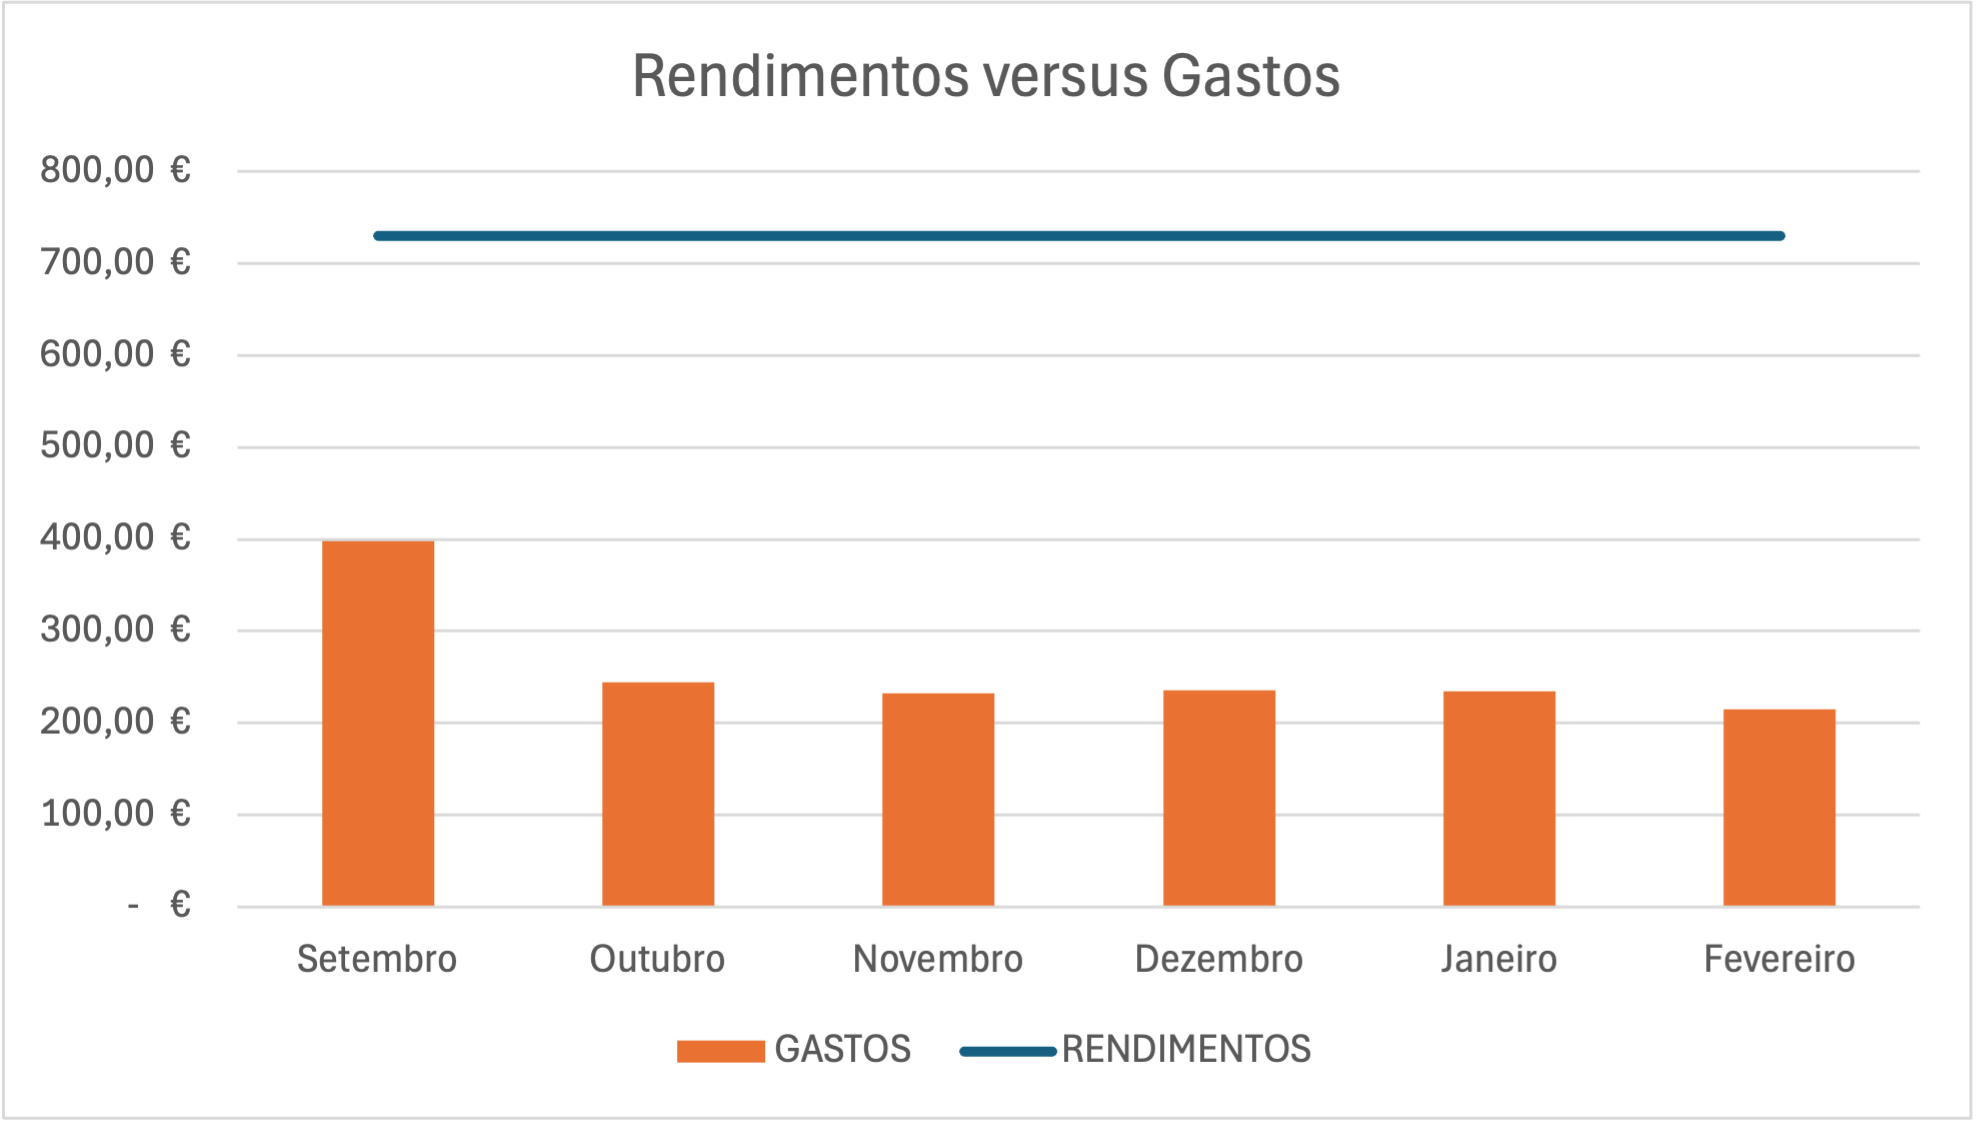
\includegraphics[scale=.55]{gráfico_rendimentosVSgastos.png}
\label{gráfico de barras}
\end{center}
\end{figure}

\begin{figure}[H]
\begin{center}
\caption{Despesas em percentagem}
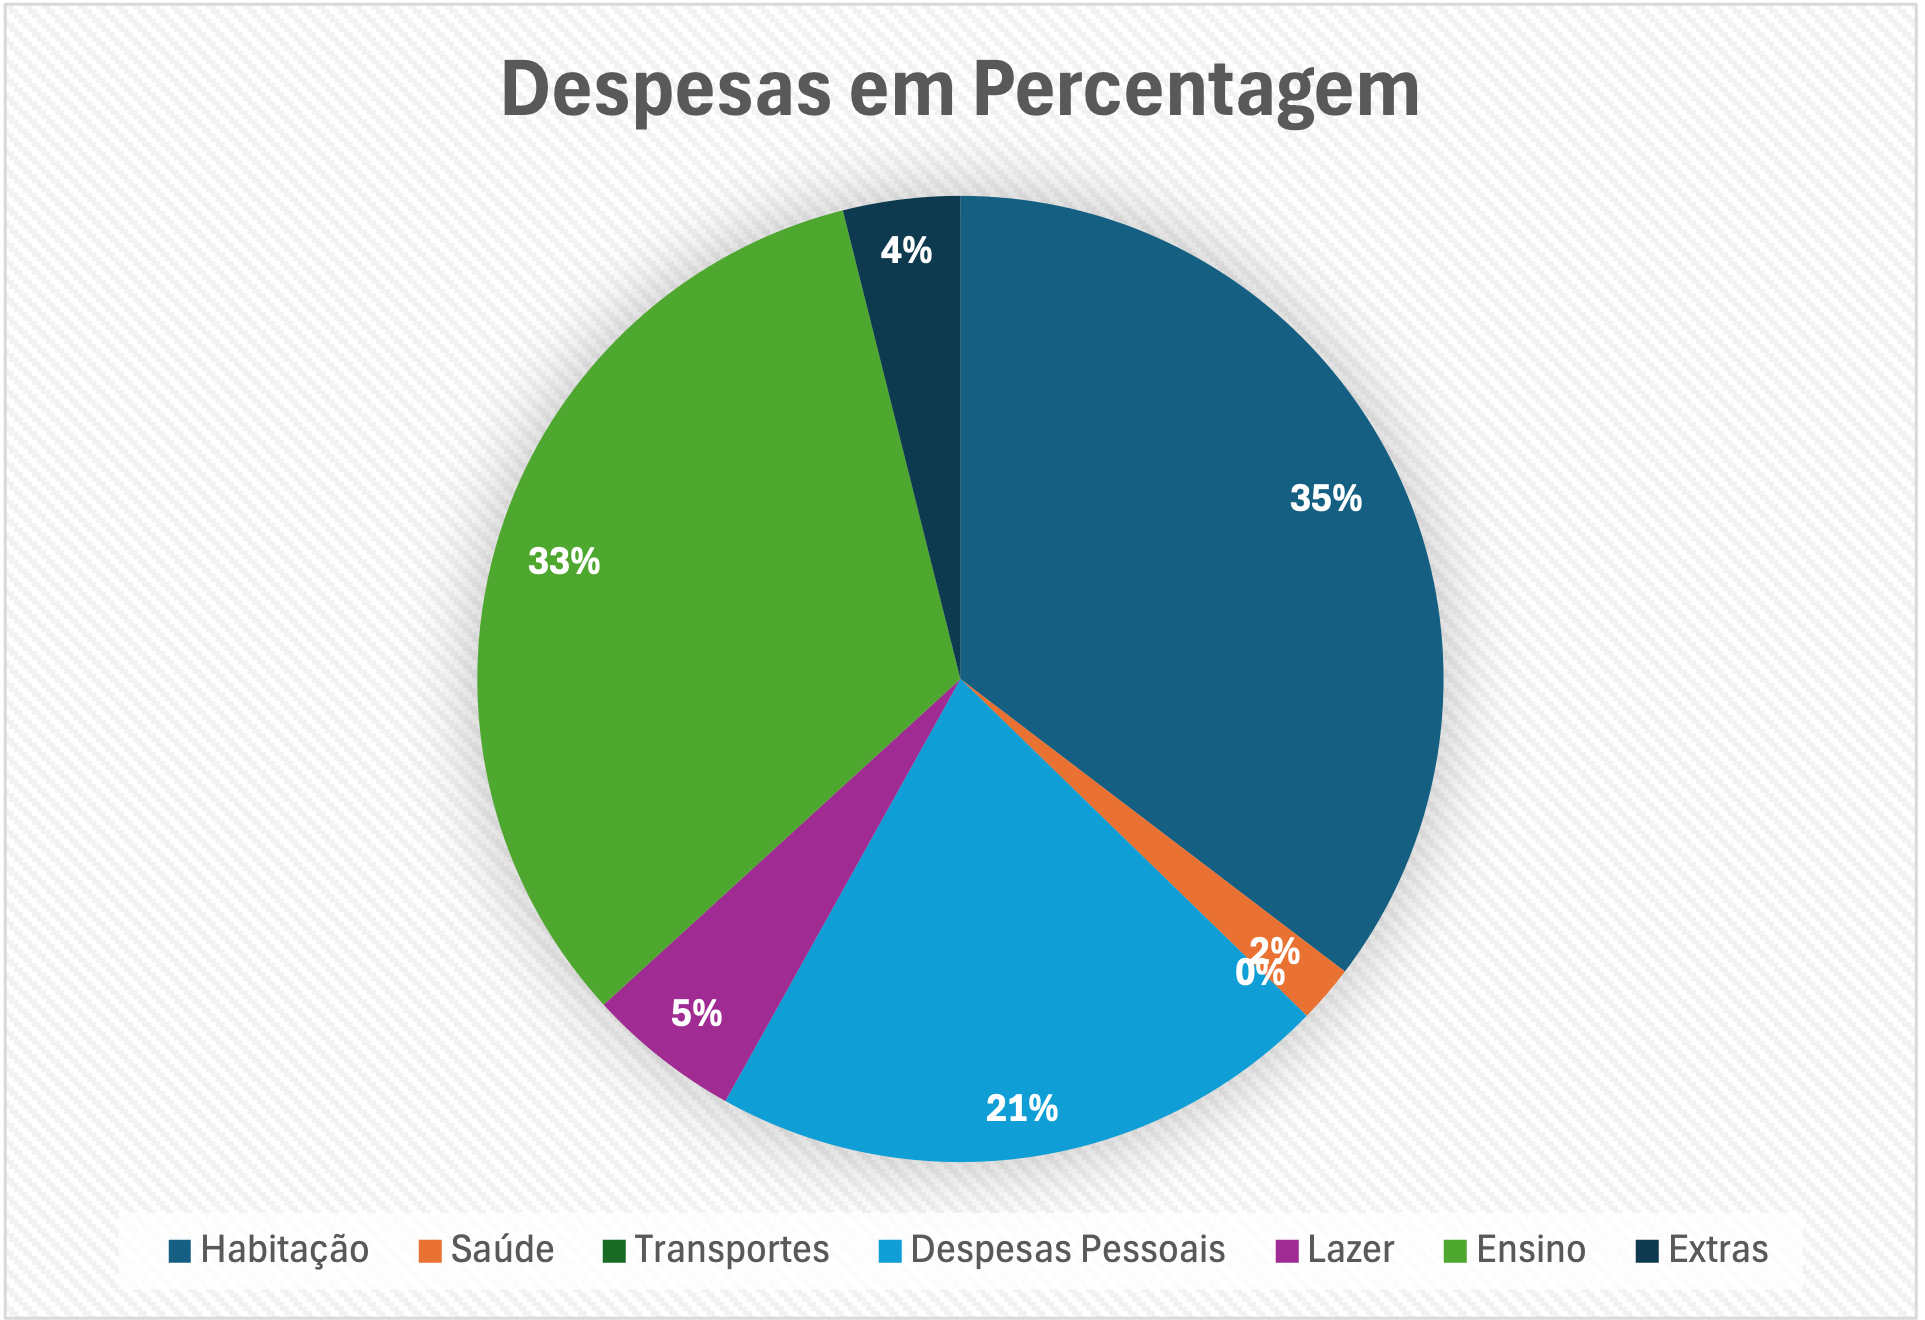
\includegraphics[scale=.55]{despesasEmPercentagem.png}
\label{gráfico circular}
\end{center}
\end{figure}

\newpage
\section{Conclusão}
Como se pode observar, a partir da tabela \ref{tabela planeamento}, sistematizar o orçamento por temas (onde se totalizam os sub-temas) e meses, traz organização e maior agilidade na gestão do nosso dinheiro. \newline\newline Na tabela \ref{tabela resumo}, somam-se todos os gastos da tabela \ref{tabela planeamento} no parâmetro "Gastos". Esta tabela, como o nome indica, resume os gastos da tabela \ref{tabela planeamento}. Em cada mês, através da diferença entre os rendimentos e os gastos, obtém-se o saldo do mês. Já o saldo acumulado indica a soma do que sobra de mês a mês (exemplo: o saldo acumulado do mês de outubro é a soma do saldo do mês de setembro e do saldo do mês outubro, e assim por diante). \newline\newline Pelo gráfico \ref{gráfico de barras}, podemos observar que, no meu caso, os rendimentos estiveram sempre bastante acima dos gastos, significando que obtive grande quantidade de saldo positivo todos os meses, logo, bastante saldo acumulado mensal. \newline\newline O gráfico \ref{gráfico circular} ilustra a tabela \ref{tabela As Contas}, dando este uma perspetiva visual e em percentagem da mesma. 
\newline\newline Tendo em conta este estudo, no meu ponto de vista, é muito benéfico criar e atualizar um orçamento pessoal. Transforma a visão e a gestão financeira, podendo ficar-se mais tranquilo e despreocupado com os gastos mensais. Quanto à periodicidade de atualização, penso que seja melhor semanalmente (quando diariamente não é possível).

\newpage
\section{Bibliografia}
\begin{itemize}
\item \href{https://www.mobills.com.br/blog/financas-pessoais/tudo-sobre-financas-pessoais/}{Mobills - Tudo sobre Finanças Pessoais}
\item \href{https://blog.omie.com.br/orcamento-continuo-significado-exemplos-e-como-usar/}{Omie - Orçamento contínuo: significado, exemplos e como usar}
\end{itemize}

\end{document}

